\documentclass[12pt,a4paper]{article}
\usepackage[utf8]{inputenc}
\usepackage[T1]{fontenc}
\usepackage[french]{babel}
\usepackage[margin=1.7cm]{geometry}
\usepackage{amsmath,amssymb}
\usepackage{mathrsfs}
\usepackage{graphicx}
\usepackage{enumitem}
\usepackage{tcolorbox}
\usepackage{xcolor}
\usepackage{titlesec}
\usepackage{multicol}

\tcbuselibrary{skins}

\definecolor{bandeau}{HTML}{E8EEF7}
\definecolor{titrebleu}{HTML}{1A4FA0}

% Bandeau de titre pour chaque exercice
\newtcbox{\exobox}{
  colback=bandeau, colframe=bandeau, boxrule=0pt,
  arc=0pt, left=4pt, right=4pt, top=3pt, bottom=3pt,
  fontupper=\bfseries, width=\linewidth, halign=left
}

\newcommand{\exercice}[3]{%
  \vspace{0.15em}
  \noindent\exobox{Exercice #1 --- #2}\par
  \vspace{0.15em}
}

\pagestyle{empty}
\setlist{topsep=2pt, itemsep=3pt, parsep=0pt}
\setlength{\parskip}{2pt}

\begin{document}

\begin{center}
  {\LARGE\bfseries Contrôle --- Généralités sur les fonctions}\\[0.4em]
  {\itshape 1\textsuperscript{ère} ST2S \quad $\bullet$ \quad Durée~: 30 minutes \quad $\bullet$ \quad Calculatrice autorisée \quad $\bullet$ \quad \textbf{Sujet B}}
\end{center}

%\vspace{0.4em}
%\noindent
%\begin{tabular}{@{}p{0.5\linewidth}p{0.5\linewidth}@{}}
%Nom, Prénom~: \dotfill & Classe~: \dotfill \quad Date~: \dotfill
%\end{tabular}

\vspace{0.3em}
\noindent\textit{La qualité de la rédaction et la justification des réponses seront prises en compte dans la notation.}

% ---------------- Exercice 1 ----------------
\exercice{1}{Fonction affine}{4}
Soit $h$ la fonction définie sur $\mathbb{R}$ par $h(x) = -2x + 3$.
\begin{enumerate}[label=\alph*)]
  \item Calculer $h(2)$.
  \item Déterminer, par le calcul, l'antécédent de $-5$ par $h$.
\end{enumerate}

% ---------------- Exercice 2 ----------------
\exercice{2}{Inéquation}{3}
Résoudre dans $\mathbb{R}$ l'inéquation suivante~:
\[ 2x - 5 < 0 \]

% ---------------- Exercice 3 ----------------
\exercice{3}{Appartenance à une courbe}{4}
Soit $k$ la fonction définie sur $\mathbb{R}$ par $k(x) = -x^2+7$, et $\mathscr{C}_k$ sa courbe représentative dans un repère du plan.

Le point $G(-2~;~3)$ appartient-il à $\mathscr{C}_k$~? Justifier la réponse par le calcul.

% ---------------- Exercice 4 ----------------
\exercice{4}{Lecture graphique}{9}
Soit $f$ la fonction représentée par la courbe $\mathscr{C}_f$ ci-dessous, définie sur l'intervalle $[-3~;~4]$.

\begin{center}
  \vspace{-2pt}
  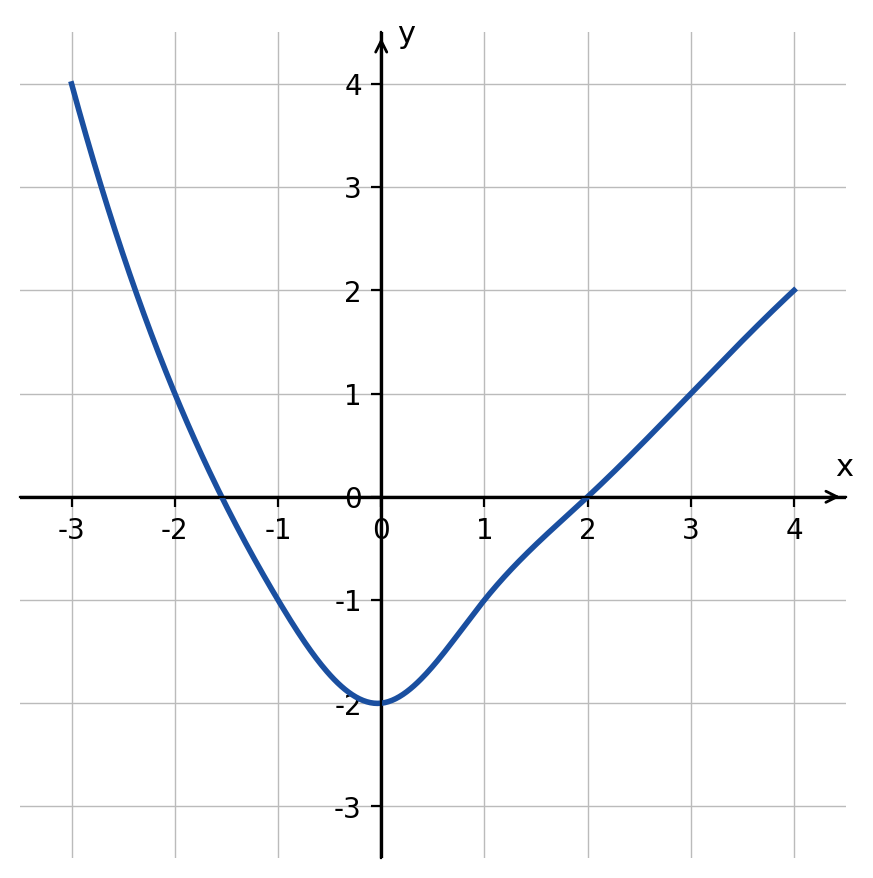
\includegraphics[width=6.3cm]{courbe_f_B.png}
  \vspace{-4pt}
\end{center}

\begin{enumerate}
  \item Donner l'image de $0$ par $f$, puis traduire cela par une égalité.
  \item Donner l'image de chacun des réels suivants~: $-1$~; $2$~; $4$.
  \item Donner un antécédent par $f$ de chacun des réels suivants~: $1$~; $2$.
  \item Résoudre graphiquement les équations suivantes~:
  \begin{enumerate}[label=\alph*.]
    \item $f(x) = -2$
    \item $f(x) = -1$
  \end{enumerate}
  \item Résoudre graphiquement l'inéquation~: $f(x) \geqslant 1$
\end{enumerate}

\end{document}
